%%%%%%%%%%%%%%%%%%%%%%%%%%%%%%%%%%%%%%%%%
% Journal Article
% LaTeX Template
% Version 1.4 (15/5/16)
%
% This template has been downloaded from:
% http://www.LaTeXTemplates.com
%
% Original author:
% Frits Wenneker (http://www.howtotex.com) with extensive modifications by
% Vel (vel@LaTeXTemplates.com)
%
% License:
% CC BY-NC-SA 3.0 (http://creativecommons.org/licenses/by-nc-sa/3.0/)
%
%%%%%%%%%%%%%%%%%%%%%%%%%%%%%%%%%%%%%%%%%

%----------------------------------------------------------------------------------------
%	PACKAGES AND OTHER DOCUMENT CONFIGURATIONS
%----------------------------------------------------------------------------------------

\documentclass[10pt]{article} % Single column

%\documentclass[twoside,twocolumn]{article} % Two column

\usepackage{blindtext} % Package to generate dummy text throughout this template 

\usepackage[sc]{mathpazo} % Use the Palatino font
\usepackage[T1]{fontenc} % Use 8-bit encoding that has 256 glyphs
\linespread{1.05} % Line spacing - Palatino needs more space between lines
\usepackage{microtype} % Slightly tweak font spacing for aesthetics

\usepackage[spanish]{babel} % Language hyphenation and typographical rules

\usepackage[hmarginratio=1:1,top=32mm,columnsep=20pt]{geometry} % Document margins
\usepackage[hang, small,labelfont=bf,up,textfont=it,up]{caption} % Custom captions under/above floats in tables or figures
\usepackage{booktabs} % Horizontal rules in tables

\usepackage{lettrine} % The lettrine is the first enlarged letter at the beginning of the text

\usepackage{enumitem} % Customized lists
\setlist[itemize]{noitemsep} % Make itemize lists more compact

\usepackage{abstract} % Allows abstract customization
\renewcommand{\abstractnamefont}{\normalfont\bfseries} % Set the "Abstract" text to bold
\renewcommand{\abstracttextfont}{\normalfont\small\itshape} % Set the abstract itself to small italic text

\usepackage{titlesec} % Allows customization of titles
\renewcommand\thesection{\Roman{section}} % Roman numerals for the sections
\renewcommand\thesubsection{\roman{subsection}} % roman numerals for subsections
\titleformat{\section}[block]{\large\scshape\centering}{\thesection.}{1em}{} % Change the look of the section titles
\titleformat{\subsection}[block]{\large}{\thesubsection.}{1em}{} % Change the look of the section titles

\usepackage{fancyhdr} % Headers and footers
\pagestyle{fancy} % All pages have headers and footers
\fancyhead{} % Blank out the default header
\fancyfoot{} % Blank out the default footer
\fancyhead[C]{Dise\~no y An\'alisis de Algoritmos. \textbf{Proyecto \# 1: La Pelota}} % Custom header text
\fancyfoot[RO,LE]{\thepage} % Custom footer text

\usepackage{titling} % Customizing the title section

\usepackage{hyperref} % For hyperlinks in the PDF

\usepackage{graphicx} % For images

\usepackage{pifont} % bullets

\usepackage{amsmath}



% Keywords command
\providecommand{\keywords}[1]
{
	\small	
	\vspace{0.5em}
	\noindent \textbf{\textit{Palabras clave --- }} #1
}


%----------------------------------------------------------------------------------------
%	TITLE SECTION
%----------------------------------------------------------------------------------------

\setlength{\droptitle}{-4\baselineskip} % Move the title up

\pretitle{\begin{center}\Huge\bfseries} % Article title formatting
	\posttitle{\end{center}} % Article title closing formatting
\title{\normalsize{Dise\~no y An\'alisis de Algoritmos }\\
	\Huge\bfseries Proyecto \# 1: La Pelota \\
} % Article title
\author{% 
	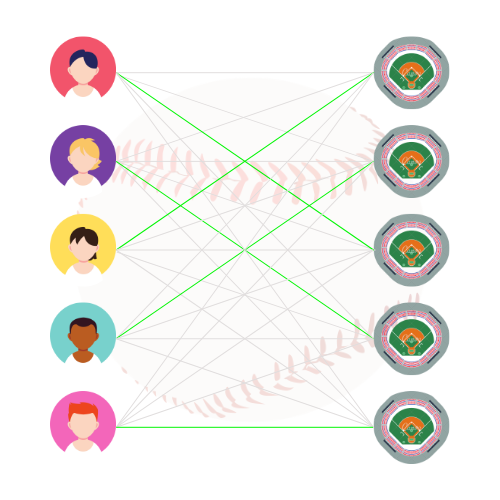
\includegraphics[width=15em]{logo.png}\\
	Laura Victoria Riera P\'erez\\
	Mari\'e del Valle Reyes \vspace{1em} \\
	\small Cuarto a\~no. Ciencias de la Computaci\'on. \\ % institution
	\small Facultad de Matem\'atica y Computaci\'on, Universidad de La Habana, Cuba \\ % institution
}
\date{\footnotesize \today } % Leave empty to omit a date


% Abstract configurations
\renewenvironment{abstract}
{\small
	\begin{center}
		\bfseries \abstractname\vspace{-.5em}\vspace{0pt}
	\end{center}
	\list{}{
		\setlength{\leftmargin}{1.5cm}%
		\setlength{\rightmargin}{\leftmargin}%
	}%
	\item\relax}
{\endlist}

\usepackage{amsthm}
\usepackage{amssymb}
\usepackage{todonotes} % \TODO
\usepackage{listings} % Code listings
\usepackage{xcolor}

\definecolor{backcolour}{rgb}{0.95,0.95,0.92}

\newcommand{\csl}[1]{\colorbox{backcolour}{\texttt{#1}}}

\newcommand{\imgcaption}[2]{\tiny \textbf{Figura #1.} #2.}

\newcommand{\mgc}[2][]{\colorbox{backcolour}{\texttt{\_\_#2\_\_#1}}}

\newcommand{\mgccapt}[1]{\texttt{\_\_#1\_\_}}

\newtheorem{thm}{Teorema}
\newtheorem{mydef}{Definici\'on}%[section]

\renewcommand{\qedsymbol}{\rule{0.7em}{0.7em}}

% Hyperlinks configurations
\hypersetup{
	colorlinks=true,
	linkcolor=black,
	filecolor=magenta,      
	urlcolor=cyan,
	pdftitle={Overleaf Example},
	pdfpagemode=FullScreen,
}

%----------------------------------------------------------------------------------------

\begin{document}
	% Print the title
	\maketitle
	
	%----------------------------------------------------------------------------------------
	%	ARTICLE CONTENTS
	%----------------------------------------------------------------------------------------
	
	\section{Repositorio del proyecto}
	
	\begin{center}
		\href{https://github.com/computer-science-crows/algorithms-design-and-analysis}{https://github.com/computer-science-crows/algorithms-design-and-analysis}
	\end{center}

	\section{Definici\'on inicial del problema} 
	
	Para un campeonato de pelota, el manager debe elegir de un conjunto de $ n $ personas, a su equipo de $ p $ jugadores, y a $ k $ espectadores especiales para que suban la moral del equipo.
	De cada persona $ i $, el manager conoce el valor que aporta a la moral del equipo $ a_i $ y el valor que aporta siendo situado en la posici\'on $ j $, $ s_{i,j} $. 
	Determine una alineación entre jugadores en el campo y espectadores de forma que el equipo tenga la mayor cantidad de valor acumulado posible.
	
	\section{Definici\'on en t\'erminos matem\'atico - computacionales}
	
	\subsection{Preliminares}
	
	\begin{mydef}
		Grafo bipartito
	\end{mydef}
	
	\begin{mydef}
		Grafo bipartito completo
	\end{mydef}
	
	\begin{mydef}
		Para un grafo no dirigido $G = (V,E)$, un emparejamiento es un subconjunto de aristas $M \in E$ tal que cada v\'ertice en $V$ tiene al menos una a arista incidente en $M$.
	\end{mydef}

	\begin{mydef}
		Otras definiciones
	\end{mydef}

	\begin{mydef}
		Camino M-alternativo
	\end{mydef}
	
	\begin{mydef}
		Camino M-aumentativo
	\end{mydef}
	
	\subsection{Problema de asignaci\'on}
	
	\section{Posibles soluciones investigadas}
	
	\section{L\'inea de pensamiento}
	\subsection{Max flow min cut para mayor emparejamiento}
	No maximiza segun costos de aristas
	
	Se decidio implementar el Hungarian \todo{referencia al introduction} por ser la solucion existente que resuelve lo pensado. 
	
	
	\section{Hungarian algorithm}
	Dado un grafo bipartito completo ponderado $G = (V,E)$, donde $V = L \cup R$. Se asume que los v\'ertices de los conjuntos $L$ y $R$ contienen $n$ v\'ertice cada uno, por tanto el grafo contiene $n^2$ aristas. Para $l \in L$ y $r \in R$, se denota el peso de la arista $(l,r)$ como $w(l,r)$, lo cual representa ganancia de emparejar el v\'ertice $l$ con el v\'ertice $r$.
	
	El objetivo es encontrar el emparejamiento perfecto $M*$ cuyas aristas tengan el peso m\'aximo total de todos los emparejamientos perfectos posibles. 
	
	Sea $w(M) = \sum_{(l,r) \in M} w(l,r)$ el peso total de las aristas en el emparejamiento $M$, se quiere encontrar el emparejamiento perfecto $M^*$ tal que,
	\[w(M*)=\text{max}\{w(M):M \text{ es un emparejamiento perfecto}\}\].
	
	A encontrar un emparejamiento perfecto de peso m\'aximo se le llama \textbf{problema de asignaci\'on}. Una soluci\'on del problema de asignaci\'on es un emparejamiento perfecto que m\'aximice el costo total.
	
	Aunque se pueden enumerar los $n!$ emparejamientos perfectos pra resolver este problema, existe un algoritmo llamado \textbf{algoritmo H\'ungaro} que lo resuelve m\'as r\'apido. En vez de trabajar con un grafo bipartito completo $G$, el algoritmo H\'ungaro trabaja con un subgrafo de $G$ llamado \textbf{subgrafo de igualdad}. El subgrafo de igualdad cambia en el tiempo y tiene la propiedad que cualquier emparejamiento perfecto en el subgrafo de igualdad es tambi\'en una soluci\'on \'optima del problema de asignaci\'on.
	
	El subgrafo de igualdad depende de asignar un atributo $h$ a cada v\'ertice. El atributo $h$ se llama \textbf{etiqueta} del v\'ertice. 
	
	Se dice que $h$ es un \textbf{etiquetado de vértice factible} de $G$ si $l.h + r.h \geq w(l,r)$ para todo $l \in L$ y $r \in R$.
	
	Un etiquetado de v\'ertice factible siempre existe, como el \textbf{etiquetado de v\'ertice por defecto} dado por
	\begin{align}
		l.h &= \text{max} \{w(l,r):r \in R\} &\text{para todo } l \in R,\\
		r.h &= 0 &\text{para todo } r \in R 
	\end{align}

	Dado un eqiquetado de v\'ertice factible $h$, el \textbf{subgrafo de igualdad} $G_h = (V, E_h)$ de $G$ consiste de los mismos v\'ertice de $G$ y el subconjunto de aristas $E_h = \{(l,r) \in E: l.h + r.h = w(l,r)\}$.
	
	\begin{thm}
		
		Sea $G=(V,E)$, donde $V = L \cup R$, un grafo bipartito completo donde cada arista $(l,r) \in E$ tiene peso $w(l,r)$. Sea $h$ un etiquetado de v\'ertice factible de $G$ y $G_h$ el subgrafo de igualdad de $G$. Si $G_h$ contiene un emparejamiento perfecto $M^*$, entonce $M^*$ es una soluci\'on \'optima del problema de asignaci\'on $G$.
		
	\end{thm}

	\begin{proof}
		Si $G_h$ tiene un emparejamiento perfecto $M^*$, entonces debido a que $G_h$ y $G$ tienen el mismo conjunto de v\'ertices, $M^*$ es tambi\'en un emparejamiento perfecto en $G$. Debido a que cada arista de $M^*$ pertenece a $G_h$ y cada v\'ertice tiene exactamente una arista incidente del emparejamiento perfecto, entonces se tiene
		
		\begin{align}
			w(M*) &= \sum_{(l,r) \in M*} w(l,r)\\
			&= \sum_{(l,r) \in M^*}(l.h + r.h) &\text{(porque todas las aristas de $M^*$ pertenecen a $G_h$)}\\
			&= \sum_{l \in L}l.h + \sum_{r \in R} r.h &\text{(porque $M^{*}$ es un emparejamiento perfecto)}\\
		\end{align} 
		
		Sea $M$ un emparejamiento perfecto cualquiera de $G$, se tiene
		
		\begin{align}
			w(M) &= \sum_{(l,r) \in M} w(l,r)\\
			&\leq \sum_{(l,r) \in M} (l.h + r.h) &\text{(porque $h$ es un etiquetado de v\'ertice factible)}\\
			&= \sum_{l \in L} l.h + \sum_{r \in R} r.h &\text{(porque $M$ es un emparejamiento perfecto)}
		\end{align}
		Entonces se tiene
		\begin{equation}
			w(M) \leq \sum_{l \in L} l.h + \sum_{r \in R} r.h = w(M^*),
		\end{equation}
		por tanto $M^*$ es un emparejamiento perfecto de m\'aximo costo en $G$.
	\end{proof}
	
	\subsection{Correctitud}
	
	\subsection{Complejidad Temporal}
	
	\subsection{Complejidad Espacial}
	
	\section{Generador de casos de prueba}
	
	\section{Tester}
	
	\section{Otras soluciones y demostraciones}
	
	\section{Comparaci\'on de soluciones implementadas}
	
	\begin{thebibliography}
		a
		\bibitem{introduction} Cormen, Thomas H. y otros. \emph{Introduction to Algorithms}. 
		The MIT Press.
		4ta Edici\'on.		
		Cambridge, Massachusetts.
		2022.
	\end{thebibliography}
\end{document}


